\subsection{Blended Isogeometric Discontinuous Galerkin (BIDG) Method}
\label{sec:isogeometric}

% DG
The discontinuous Galerkin (DG) method is a finite element method (FEM) that is appealing in
aspects of its computational efficiency on modern architectures,
particularly in the context of explicit wave propagation.  In this context, DG allows for localization of
finite element stencils (e.g nearest edge/face neighbors) in such a way that dynamic problems lead to block
diagonal matrix systems, providing the capability to compute solutions at high order accuracy on sparse meshes with large memory throughput \cite{Klockner20097863}.

% Iso
In isogeometric analysis, geometric shape functions and finite element test functions are chosen as isogeometric basis functions (e.g. NURBS or splines) \cite{Riesenfeld20151054}.  This choice is made to address the so-called design-to-analysis bottleneck, where the engineering design community utilizes computer aided design (CAD) technologies to parameterize complicated geometries, but in such a way that resulting seams and gaps in the meshes make them impossible to perform finite element analysis (FEA) on.  IGA solves this problem by building into CAD programs isogeometric basis functions that lead to CAD meshes that are analysis suitable.  Moreover, it is known that traditional efforts to deal with complicated geometric domains, such as heavily refining linear meshes are using isoparametric elements, can lead to ``geometric variational crimes.''    In fact, in many applications, geometric sensitivities dominate error behavior \cite{Michoski2016658,Wirasaet2015597,Fahs:2011:IAH:2003056.2003066,Toulorge_a2d},
necessitating geometrically consistent meshes for accurate solutions at high
polynomial order.


The BIDG algorithm developed in \cite{Michoski2016658} merges key capabilities
offered by both IGA and DG methods.  In BIDG different basis functions are used to parameterize the geometry than to solve for the DG method.  For the geometry piecewise rational Bernstein-B\'{e}zier basis functions are used, and for the DG basis piecewise discontinuous polynomials are used.  What this provides is the ability to exactly parameterize complex geometries, while still being able to utilize the small localized stencils from DG methods.   A set of geometric transformations between the DG and IGA bases is then easily established, up to a constraint on the conditioning of the IGA elements of the mesh. 
Recently automation tools for complex geometric domains have also been developed for BIDG on triangles in two dimensions \cite{Engvall2016378} and generalized elements in three dimensions \cite{EngvallPress}.  This allows for meshes that exactly
preserve underlying geometry in real-world designs, including both arbitrarily
smooth and discontinuous features. The resulting BIDG method is an inherently high-order method that is amenable to $hp$-adaptive schemes, and shows requisite and theoretically rigorous super-exponential convergent behavior.


One of nuances of solving curvilinear systems is the relatively heavy storage requirements.  In linear systems the element coordinate transforms are affine, thus the geometric factors are constant over elements, and can be factored out of stiffness and mass matrix calculations.  In the case of curvilinear elements however this is not the case, where the geometric transforms have elementwise dependencies.  This is particularly problematic in isoparametric methods, where the degree of the geometric basis tends to increase with the solution basis \cite{doi:10.1137/120899662}.  However, in the BIDG method, because the geometric parameterization is isogeometric, the method is generally speaking a subparametric method, since the exact geometry can be preserved at a lower rational degree than the solution basis  \cite{Michoski2016658}.  What this leads to is a larger storage requirement for the mesh itself at low polynomial degree $\ell$ and a smaller one at higher polynomial degree.  A number of solutions to this heavy storage problem have been presented in the literature for isoparametric methods \cite{doi:10.1137/120899662}, though these have not yet been tested in BIDG.


\begin{figure}
\begin{center}
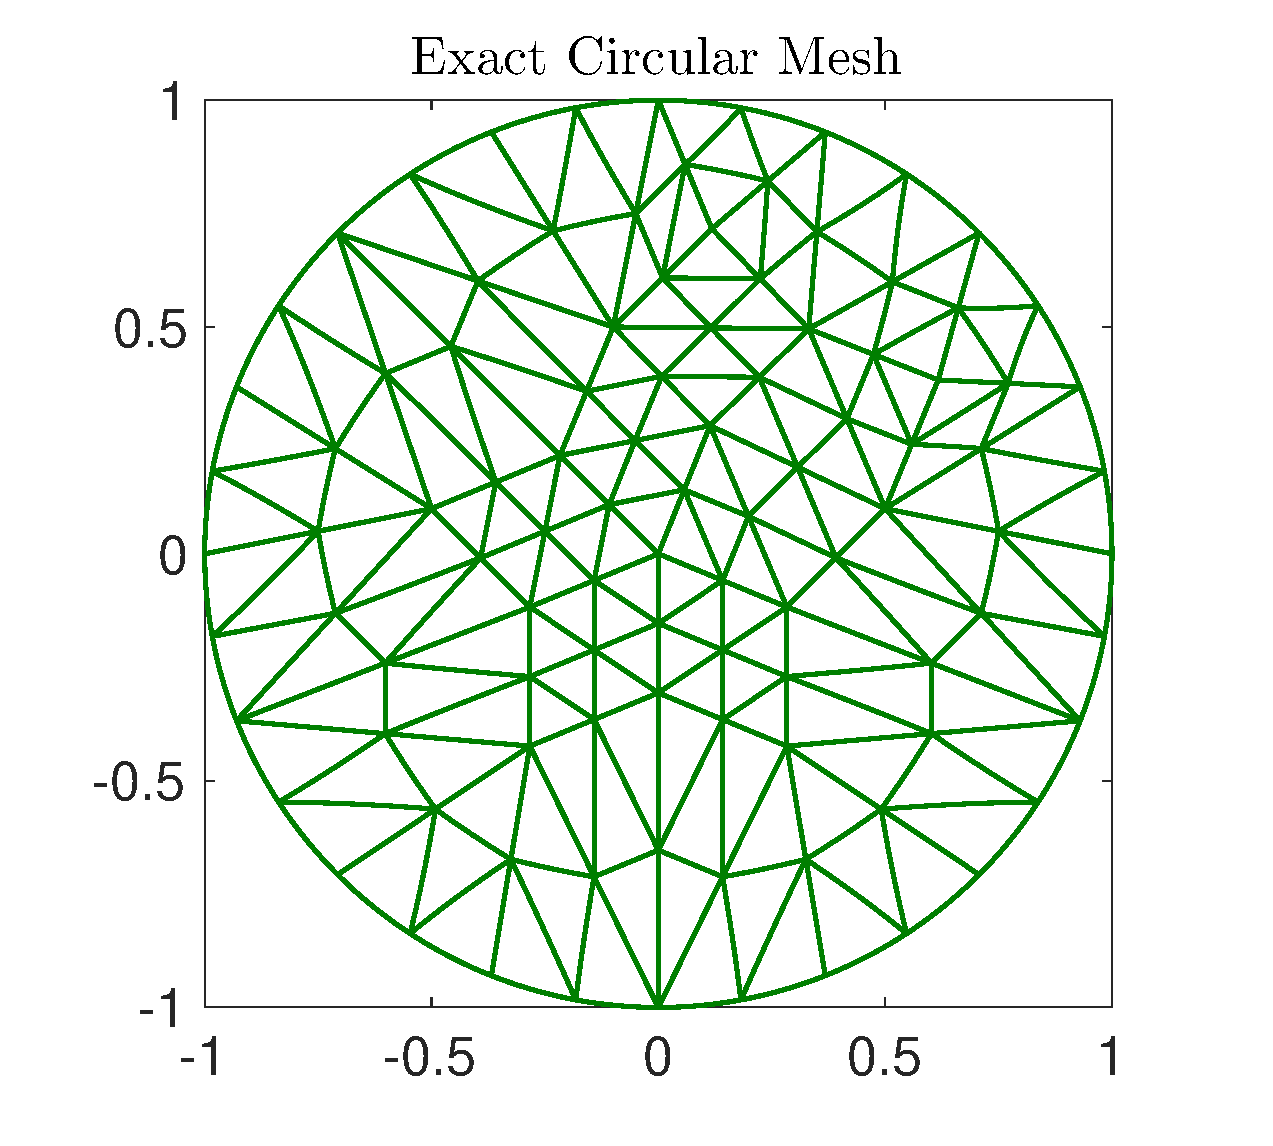
\includegraphics[width=0.8\linewidth]{./bidg_data/168_circ}
\end{center}
\vspace*{-.5cm}
\caption{Exact b\'{e}zier circular mesh used in the scaling study.}
\label{fig:168_circ}
\end{figure}

The software package ArcSyn3sis implements the BIDG method and it is used here
for the scaling study on the KNL architecture. For our strong scaling test we solve the first-order acoustic wave equation:
\begin{equation}
  \label{awe}
  \frac{\partial p}{\partial t} + \nabla\cdot \boldsymbol{u} = 0, \quad
  \frac{\partial\boldsymbol{u}}{\partial t} + \nabla p = 0,
\end{equation}
where $\boldsymbol{u}=(u_x,u_y)$ is the velocity, and $p$ the pressure. The following semidiscrete block diagonal system results:
\[
  \left( v, \frac{ \partial A}{\partial t} \right)_{\Omega_{i}} =
  V_{\Omega_{i}}+S_{\partial\Omega_{i}}
\]
for $A = (p,\boldsymbol{u})$, $V_{\Omega_{i}}$ a volume kernel that has only
elementwise dependencies, and $S_{\partial\Omega_{i}}$ a surface kernel that
depends on inter-element communication through classical upwinding
\cite{Michoski2014898}.  The resulting system can be understood as a globally sparse block-matrix, where the blocks are dense, thus motivating the use of a many-core architecture for execution.  The implementation utilizes the Open Concurrent Compute Abstraction (OCCA) library \cite{MedinaPress}.  The OCCA library abstracts multiple threading back-ends (OpenMP, OpenCL, and CUDA) using C preprocessor macros.

%% The solution kernel subsequently The volume integral can be written in three nested
%% loops; the outer looping over elements, and two inner loops over degrees of
%% freedom in the DG basis.  The surface intergral similarly loops over elements,
%% but then due to an additional interpolation step from the isogeometric
%% transformation, extends one of these nested loops over the quadrature degrees
%% of freedom for curved edges.  The resulting linear system that is solved,
%% $Fx = b$ admits an attractive block-diagonal structure,
%% \begin{equation}
%%   F = \begin{pmatrix}
%%     F_1 & 0 & \cdots & 0 \\
%%     0 & F_2 & \cdots & 0 \\
%%     \vdots & & \ddots & \vdots \\
%%     0 & 0 & \cdots & F_n \\
%%   \end{pmatrix},
%% \end{equation}


\begin{figure}
\begin{center}
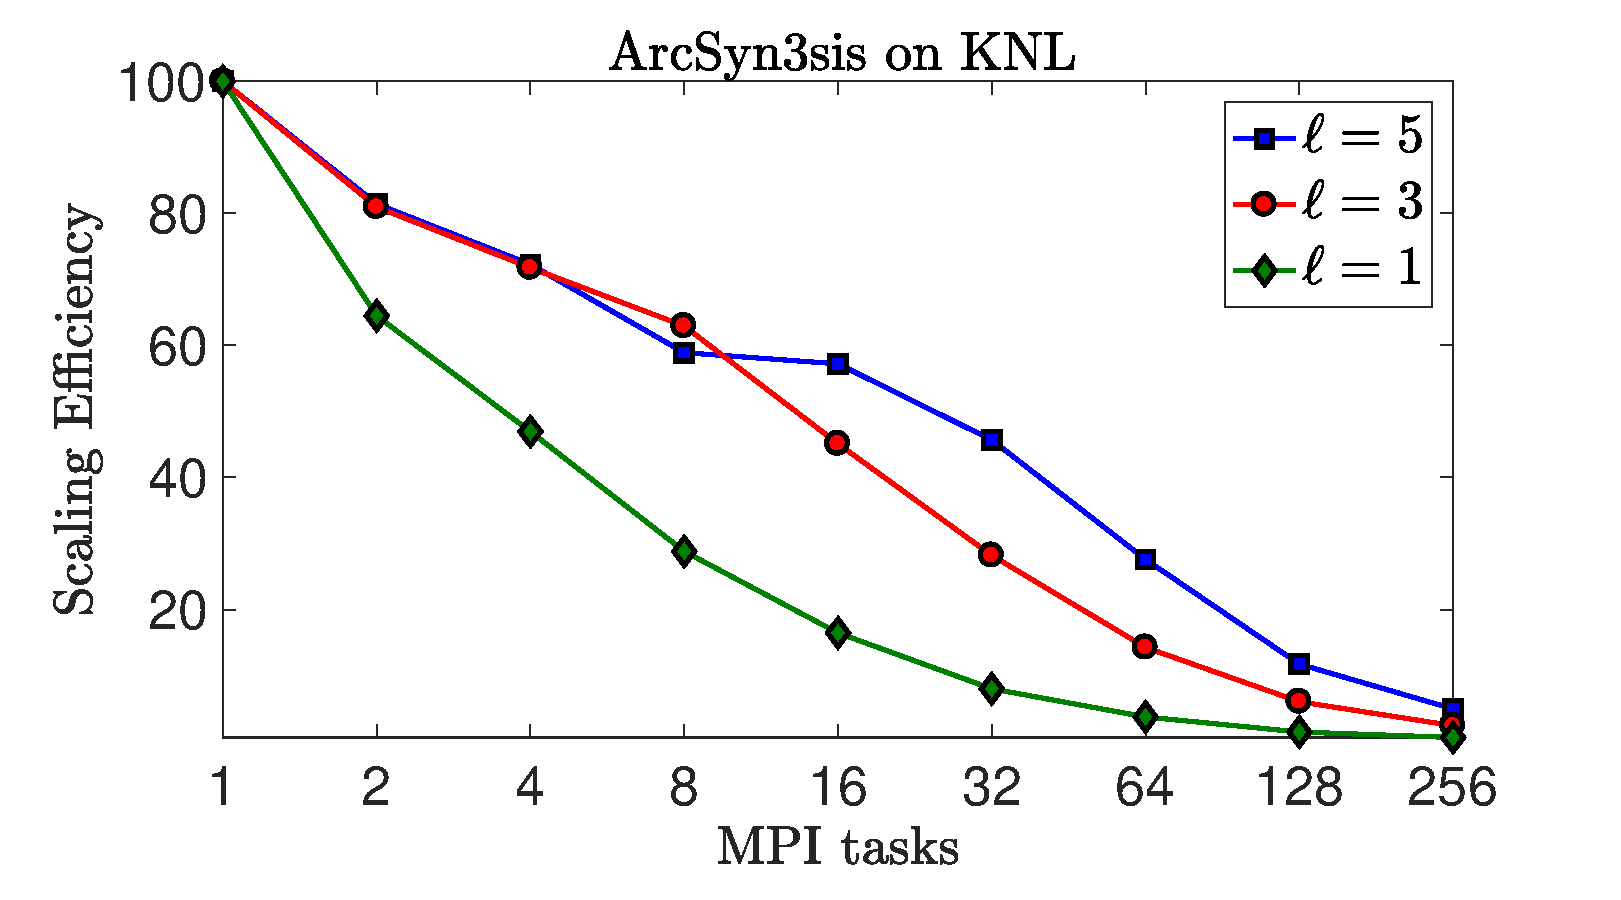
\includegraphics[width=0.99\linewidth]{./bidg_data/2nd_try/scaling}
\end{center}
\vspace*{-.5cm}
\caption{Strong scaling of the ArcSyn3sis BIDG kernel on KNL nodes run on
isogeometric 168 element mesh, and shown at different polynomial order $\ell$.}
\label{fig:bidg_scaling}
\end{figure}


% The OCCA kernel implements macro-based just-in-time code
% generation so that the platform target can be identified at runtime.  Threaded
% barriers are also set in the application kernel to allow for thread-based
% granularity, giving more flexibility during code optimization.  The
% implementation of the ArcSyn3sis kernel using OCCA allows for aliasing, of e.g.
% flattened cache-line boundary aligned arrays, such that data structures can be
% called more intuitively (e.g.  a 4-tensor can be called as a four array,
% instead of indexed as a flattened contiguous one array).

The results of the basic scaling study are shown in
Fig.~\ref{fig:bidg_scaling}, where the strong scaling efficiency $e_{n}$ for
$n$ MPI tasks is defined as $e_{n}= [t_{1}/(nt_{n})]\times 100\%$, and $t_n$ is the time to
completion. These preliminary results seem to indicate improved scaling as a function of polynomial order $\ell$, which is consistent with the theoretical
behavior of the algorithmic intensity of DG algorithms.  However, this is
clearly not enough evidence to be certain that such scaling is being observed.
In particular, on this mesh we see an efficiency saturation above $\ell>5$.
Moreover, since the mesh itself has only 168 elements, the number of threads
eventually exceeds the number of elements, making for some intriguing questions
regarding the observed behavior.  In order to fully understand the observed behavior and
optimize the code appropriately, a more extensive study is required, including
%a streams
%
%NM-- why streams? Streams is just a memory bandwidth benchmark. If this is
%     expected to be the bottleneck, I would directly address that in the text.
%CM -- Nick, sorry, I don't understand your point.  I don't know what the bottleneck is because I have not done comprehensive tests, so I can't rule out a bottleneck until I run the tests.  All I can do is guess.  Memory bandwidth may very well be causing a problem, and the vector kernels should be tested.  On the other hand, I think the roofline model would cover this too, so we can delete it if you prefer?
%benchmark \cite{McCalpin1995} and
a roofline performance test
\cite{Williams:2009:RIV:1498765.1498785}.

%
% NM --- feel free to disregard anything I recommend here
%
 %yar\todo{Discuss, broadly, what class of problems this resides in and why humanity works on it}

%% yar2\todo{some basic intro to the linear algebra you are doing}

%% yar3\todo{any nuances of porting to MIC?}

%% yar4\todo{discussion of scalability observed}

%Finally, some discussion is needed: is DG ameniable to MICs? Vs typical CPUs? I
%naively guess so, since you can essentially vectorize several of the
%activities.
